% Rebuild the committed PDF with: bash scripts/build-walkthrough.sh
% Optional maintainer source. Readers use docs/clutta-walkthrough.pdf.
% Authoring tools only: XeLaTeX, Latin Modern fonts, Inkscape, and Poppler.
% No authoring tools are required to read the PDF or run the lab.
% Colors match https://clutta.io/ stylesheet tokens, checked 2026-10-02.
% This is a walkthrough, not a replay or a fabricated Clutta evidence receipt.
\documentclass[10pt,a4paper]{article}
\usepackage[left=19mm,right=19mm,top=16mm,bottom=16mm]{geometry}
\usepackage{fontspec}
\setmainfont{Latin Modern Roman}
\setsansfont{Latin Modern Sans}
\setmonofont{Latin Modern Mono}[Scale=0.88]
\usepackage{graphicx,xcolor,tikz,tabularx}
\usetikzlibrary{arrows.meta}
\usepackage[unicode,colorlinks=true,urlcolor=blue,linkcolor=blue]{hyperref}
\definecolor{navy}{HTML}{001A6E}
\definecolor{blue}{HTML}{174AE5}
\definecolor{ink}{HTML}{05050A}
\definecolor{muted}{HTML}{646979}
\definecolor{line}{HTML}{D9DEEB}
\definecolor{pale}{HTML}{F4F4FF}
\hypersetup{
  pdftitle={Clutta Walkthrough},
  pdfauthor={Clutta},
  pdfsubject={A short scheduler walkthrough and hands-on Clutta lab},
  pdfkeywords={Clutta, workflow completion, scheduler, silent failure, playground},
  pdfcreator={Clutta},
  pdfdisplaydoctitle=true
}
\pagestyle{empty}
\setlength{\parindent}{0pt}
\setlength{\parskip}{0pt}
\renewcommand{\arraystretch}{1.08}
\color{ink}
\newcommand{\sectionlabel}[1]{{\sffamily\fontsize{8.5}{10}\selectfont\bfseries\color{blue}\MakeUppercase{#1}}}
\newcommand{\bodytext}[1]{{\fontsize{10.2}{14}\selectfont #1\par}}
\newcommand{\step}[4]{%
  \begin{tabularx}{\linewidth}{@{}p{8mm}X@{}}
    {\sffamily\fontsize{17}{20}\selectfont\bfseries\color{blue}#1} &
    {\sffamily\fontsize{10.8}{13}\selectfont\bfseries #2}\hfill{\fontsize{9.1}{11}\selectfont\ttfamily\color{navy}#3}\\[-0.2mm]
    & {\fontsize{10}{13.4}\selectfont #4}
  \end{tabularx}\par\vspace{3.0mm}}
\begin{document}
\begin{minipage}[c]{0.36\linewidth}
  \includegraphics[width=31mm]{clutta-logo.pdf}
\end{minipage}%
\begin{minipage}[c]{0.64\linewidth}
  \raggedleft{\sffamily\fontsize{8.5}{11}\selectfont\color{muted}SHORT WALKTHROUGH\quad /\quad HANDS-ON LAB}
\end{minipage}

\vspace{5mm}
{\fontsize{30}{33}\selectfont\bfseries\color{navy}Everything is green.\par}
{\fontsize{30}{33}\selectfont\bfseries\color{blue}The notification never arrived.\par}
\vspace{3.5mm}
\bodytext{A payment finishes, but its notification scheduler stops doing useful work. The container stays healthy. Clutta watches whether the journey finishes, not just whether the service is alive.}
\vspace{4mm}

\sectionlabel{The journey you will watch}\par\vspace{2mm}
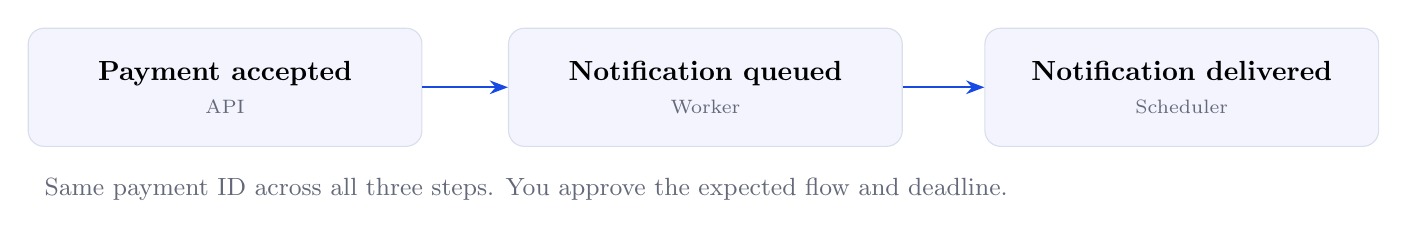
\begin{tikzpicture}[x=1mm,y=1mm,>=Stealth,inner sep=2mm]
  \node[draw=line,fill=pale,rounded corners=2mm,minimum width=50mm,minimum height=15mm,align=center,font=\fontsize{10}{12}\selectfont] (a) at (25,0) {\textbf{Payment accepted}\\{\color{muted}\scriptsize API}};
  \node[draw=line,fill=pale,rounded corners=2mm,minimum width=50mm,minimum height=15mm,align=center,font=\fontsize{10}{12}\selectfont] (b) at (86,0) {\textbf{Notification queued}\\{\color{muted}\scriptsize Worker}};
  \node[draw=line,fill=pale,rounded corners=2mm,minimum width=50mm,minimum height=15mm,align=center,font=\fontsize{10}{12}\selectfont] (c) at (146.5,0) {\textbf{Notification delivered}\\{\color{muted}\scriptsize Scheduler}};
  \draw[->,line width=0.8pt,color=blue] (a.east) -- (b.west);
  \draw[->,line width=0.8pt,color=blue] (b.east) -- (c.west);
  \node[anchor=west,font=\fontsize{8.8}{11}\selectfont,text=muted] at (0,-13) {Same payment ID across all three steps. You approve the expected flow and deadline.};
\end{tikzpicture}\par
\vspace{3mm}

\sectionlabel{Three moments. One real workflow.}\par\vspace{3mm}
\step{1}{Learn what finished looks like}{./lab start}{Generate 600 distinct fake payments through real Node.js services and PostgreSQL. Review the proposed flow and cited runs in Clutta, then approve and activate it yourself.}
\step{2}{Stop delivery. Keep health green.}{./lab break}{The lab verifies 20 fresh healthy payments before pausing the scheduler loop. A new payment misses its delivery deadline. Open the Case File linked in your terminal.}
\step{3}{Repair and verify new work}{./lab repair}{The saved notification queue drains. Open a fresh completed run in Clutta and compare all three steps. The earlier missed deadline remains in history.}

\vspace{0.5mm}
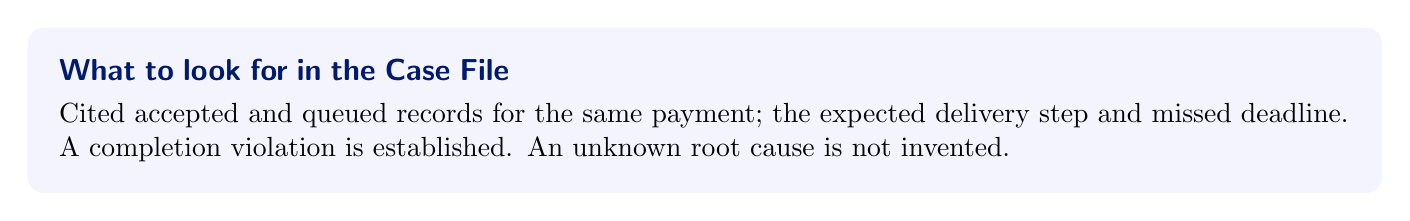
\begin{tikzpicture}
  \node[fill=pale,rounded corners=2mm,inner sep=4mm,text width=164mm,align=left] {
    {\sffamily\fontsize{10.5}{13}\selectfont\bfseries\color{navy}What to look for in the Case File}\par\vspace{1.2mm}
    {\fontsize{10}{13.4}\selectfont Cited accepted and queued records for the same payment; the expected delivery step and missed deadline. A completion violation is established. An unknown root cause is not invented.}
  };
\end{tikzpicture}\par
\vspace{4mm}

\sectionlabel{Try it in your own account}\par\vspace{2mm}
\bodytext{\href{https://app.clutta.io/signup}{Sign up for Clutta}, then follow the guide to create a lab project, get your workspace key, and open a fresh Codespace. Each step tells you what success looks like.}
\vspace{2.5mm}
\begin{tabularx}{\linewidth}{@{}X X@{}}
  \href{https://github.com/sefastech/clutta-playground/blob/main/docs/onboarding.md}{\textbf{Start the step-by-step guide $\rightarrow$}} &
  \raggedleft\href{https://codespaces.new/sefastech/clutta-playground}{\textbf{Open in Codespaces $\rightarrow$}}\tabularnewline
\end{tabularx}
\vspace{2mm}
{\fontsize{9}{12}\selectfont\href{https://github.com/sefastech/clutta-playground}{github.com/sefastech/clutta-playground}\par}
\vspace{3mm}
{\fontsize{9}{12}\selectfont Repeat the fault, fork the lab, or explore another incident with sanitized evidence in \href{https://app.clutta.io/analyze}{Analyze}. Analyze is one-time interpretation, not live monitoring or Case File creation. Finish with \texttt{./lab stop}.\par}

\vfill
{\color{line}\rule{\linewidth}{0.5pt}}\par\vspace{1.5mm}
{\fontsize{8}{10.5}\selectfont\color{muted}Real application activity; synthetic payments. No SDK, Slack, Kubernetes, or production access. Early validation: fresh-account and resume checks remain open. First-time setup and learning take longer than this short read; Codespaces usage depends on your GitHub account.\par}
\end{document}
